\subsection{Wieso macht man das?}
\begin{frame}
	\frametitle{\secname}
	\framesubtitle{\subsecname}
	
	\begin{itemize}
		\item Multicore-Systeme
			\note[item]{auch in Autos, kleine Gebrauchsgegenstände}
		\item Schnelle Ausführung
			\note[item]{Prozessorgeschwingikeit steigt nicht mehr, Anzahl dagegen schon}
	\end{itemize}
\end{frame}

\subsection{Was kann ich parallelisieren?}
\begin{frame}
	\frametitle{\secname}
	\framesubtitle{\subsecname}
	
	\begin{itemize}
		\item Sequentieller $\leftrightarrow$ Paralleler Anteil
			\note[item]{identifizierung}
		\item Logische Unabhängigkeit
			\note[item]{verschieden unabhängige Bereiche im Programm}
	\end{itemize}
\end{frame}
	
	%\lstinputlisting[language=Python, firstline=37, lastline=45]{source_filename.py}

\subsection{Beispiele}
\begin{frame}[fragile]
	\frametitle{\secname}
	\framesubtitle{\subsecname}
	
	\lstinputlisting[firstline=3]{hello.cpp}
		\note[item]{kurzes Programm, stellvertretend für viele Sequenzielle Codezeilen}
	
	\visible<2>{
		\vspace*{-1.45cm}%
		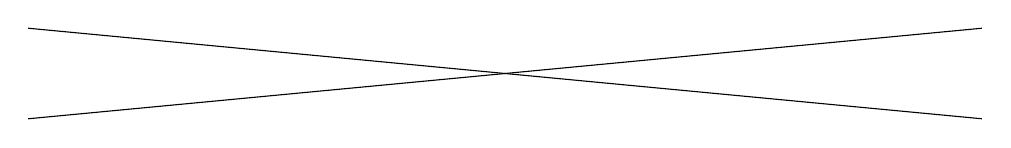
\begin{tikzpicture}
			\draw[thin](0,1.15)--(\linewidth-\pgflinewidth,0);
			\draw[thin](0,0)--(\linewidth-\pgflinewidth,1.15);
		\end{tikzpicture}
			\note[item]{}
			\note[item]{nicht oder nur sehr schlecht zu Parallelisieren}
	}
\end{frame}

\begin{frame}[fragile]
	\frametitle{\secname}
	\framesubtitle{\subsecname}
	
	\lstinputlisting[firstline=4]{section.cpp}
		\note[item]{1. Zeile von Datei ausgeben}
	
	\visible<2>{
		\vspace*{-4.4cm}%
		\begin{tikzpicture}
			\draw[thin](0,1.4)--(\linewidth-\pgflinewidth,1.4)--(\linewidth-\pgflinewidth,0)--(0,0)--(0,1.4);
		\end{tikzpicture}
		
		\vspace*{0.2cm}%
		\begin{tikzpicture}
			\draw[thin](0,1.4)--(\linewidth-\pgflinewidth,1.4)--(\linewidth-\pgflinewidth,0)--(0,0)--(0,1.4);
		\end{tikzpicture}
			\note[item]{}
			\note[item]{unabhängige Bereiche, trennen}
	}
\end{frame}

\begin{frame}[fragile]
	\frametitle{\secname}
	\framesubtitle{\subsecname}
	
	\lstinputlisting[firstline=3]{loop.cpp}
		\note[item]{Schleife (in der was ausgegeben wird)}
	
	\visible<2>{
		\vspace*{-1.5cm}%
		\hspace*{1.4cm}%
		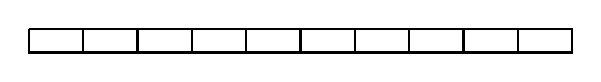
\begin{tikzpicture}
		%	\newcounter{boxnum}
			\foreach \x in {0, 1,...,9}{
				\draw[thick](1.2+0.69*\x, 0.3)--(1.888+0.69*\x, 0.3)--(1.888+0.69*\x, 0)--(1.2+0.69*\x, 0)--(1.2+0.69*\x, 0.3);
			}
		\end{tikzpicture}
			\note[item]{}
			\note[item]{Aufteilung auf beliebig viele unabhängige Einzelteile}
	}
\end{frame}

\begin{frame}[fragile]
	\frametitle{\secname}
	\framesubtitle{\subsecname}
	
	\lstinputlisting[firstline=5,lastline=12]{prefix_computation.cpp}
		\note[item]{Schleife, aber abhängig von vorherigem Ergebnis}
		\note[item]{Schwierig, nicht von allen Unterstützt}
\end{frame}

\subsection{Was nun?}
\begin{frame}
	\frametitle{\secname}
	\framesubtitle{\subsecname}
	
	\begin{itemize}
		\item Programmstruktur identifizieren
			\note[item]{Wie ist das Programm aufgeteilt}
		\item Geeignete Mittel einsetzen
			\note[item]{Hängt ab vom Ziel, Multiplattform, Embedded UND vom Programm selber, ist es schon fertig, wird ein neues geschrieben}
		\item Anpassung an Zielsystem
			\note[item]{Auf Eigenheiten des Systems eingehen, evtl. sogar auf 2,3,4 Prozessoren fest einstellen}
	\end{itemize}
\end{frame}

\subsection{Was setze ich ein?}
\begin{frame}
	\frametitle{\secname}
	\framesubtitle{\subsecname}
	
	\begin{itemize}
		\item fork
			\note[item]{sollte jeder kennen, (komplett) getrennte Prozesse}
		\item Compilerflag (-ftree-parallelize-loops)
			\note[item]{für C/C++ nur Schleifen, auch nicht alle, aber man muss nur flag setzen und kann es ausprobieren}
		\item PThread, std::thread, ...
			\note[item]{Standardwerkzeuge, C++-11}
		\item OpenMP
			\note[item]{gleich mehr}
		\item EMB$ ^2$
			\note[item]{was kann das, kleiner Vergleich}
	\end{itemize}
\end{frame}